\documentclass{article}

\usepackage{lipsum}
\usepackage[margin=1in,includefoot]{geometry}
\usepackage{graphicx}
\usepackage{float}
\usepackage[hidelinks]{hyperref}
\usepackage{amsmath}
\usepackage{amssymb}
\usepackage{color}


\usepackage[usenames,dvipsnames]{xcolor}
\usepackage{listings}







% Header and Footer Stuff
\usepackage{fancyhdr}
\pagestyle{fancy}
\fancyhead{}
\fancyfoot{}
\fancyfoot[R]{\thepage}
\renewcommand{\headrulewidth}{0pt}
\renewcommand{\footrulewidth}{0pt}


\definecolor{dkgreen}{rgb}{0,0.6,0}
\definecolor{gray}{rgb}{0.5,0.5,0.5}
\definecolor{mauve}{rgb}{0.58,0,0.82}

\lstset{
  language=VHDL,
  aboveskip=3mm,
  belowskip=3mm,
  showstringspaces=false,
  columns=flexible,
  basicstyle={\small\ttfamily},
  numbers=none,
  numberstyle=\tiny\color{gray},
  keywordstyle=\color{blue},
  commentstyle=\color{dkgreen},
  stringstyle=\color{mauve},
  breaklines=true,
  breakatwhitespace=true,
  tabsize=3
}


\begin{document}

\begin{titlepage}
	\begin{center}
	\begin{align*}
	
\includegraphics[height=1.75in]{logo.png}
	\end{align*}


	
	\line(1,0){300}\\
	[0.25in]
	\huge{\bfseries Tutorial 6 }\\
	[2mm]
	\line(1,0){200}\\
	[1.5cm]
	\textsc{\LARGE Full Game}\\
	[0.75cm]
	\textsc{\Large CS4052 Computer Graphics}\\
	[7cm]	
	\end{center}
	
	
	
	\begin{flushright}
	\textsc{\large Alexandru Sulea\\
	D Stream\\
	\#12315152\\
	16 December 2016\\}
	\end{flushright}
	
\end{titlepage}
%Table of Contents Stuff%
%\tableofcontents
%\listoffigures
%\addcontentsline{toc}{section}{List of Figures}
%\listoftables
%\addcontentsline{toc}{section}{List of Tables}


\thispagestyle{empty}
\cleardoublepage
\pagenumbering{arabic}
\setcounter{page}{1}

\pagebreak
\section{Introduction}



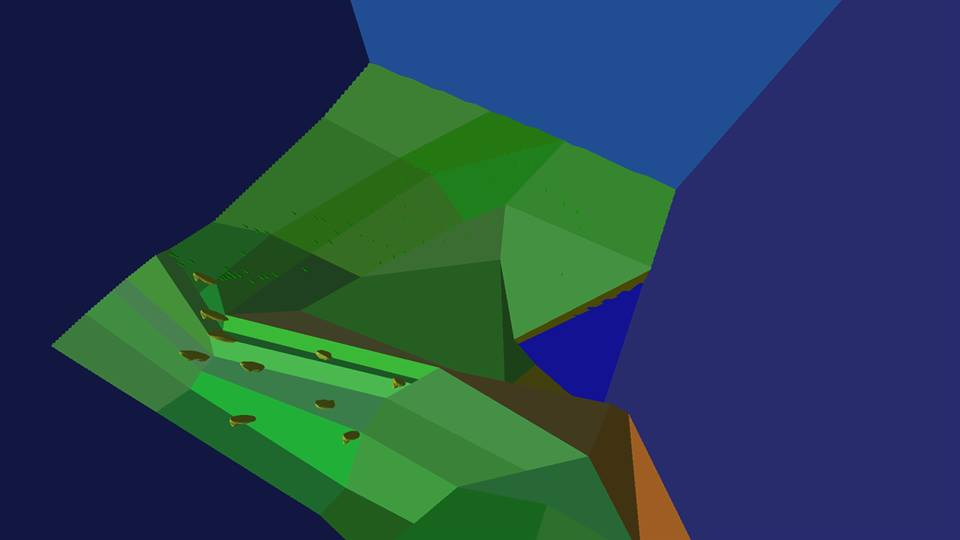
\includegraphics[height=1.75in]{pic2.PNG}


\section{User interaction and camera control}
Users can mode the player into the x-z direction and the mouse control can mode the view around.



\section{Scoring and winning/losing}
The score depends on the seconds elapsed. After each 20 second segment the life meter will decrement and the player will be closer to loosing the game. The player can put off loosing by catching the other player. This will give back one life for every time the other player is caught. There is a max of 5 lives.
\section{3D objects}
3D Models were used for this game. 


\section{Opengl Shaders for phong}
Phong lighting from the past tutorial was used to light up the game. This version of phong lighting was combined with fog.



\section{one hiararchical model}
The player has to find the other player that is hiding in the map. For help, there is a ghost above the player that is hiding so that the player can be found easily enough if the hiding spot cannot be found in time.


\section{1 texture mapped object}
All objects in the game are mapped by textures. Soil was attempted to be used but had negative effects on the game, thus std image was used for loading and displaying textures.






\section{Custom Textures}
After speaking to Emma and based on her recommendation I chose to implement textures with std lib, the custom textures were made in gimp. The texture was supposed to resemble Donald Trumps suit.
\section{Music}

Music was implemented using the standard windows c++ library The music was taken from online. The music itself was downloaded without permission from youtube. So the game will not be published publicly any time soon.





\section{user interface}
User interface is made up of the seconds counting down and also the life meter decrementing or incrementing based on wheather the player has scored. If the life meter runs out, the user will then see a game over sign.


\section{Collisons}
Collisions are implemented based on the coordinates of the main character and target character. If the two are within 2 x-z points of each other then that counts as a collision and the target is repositioned to another random spot within plus or minus 20 x or z points.
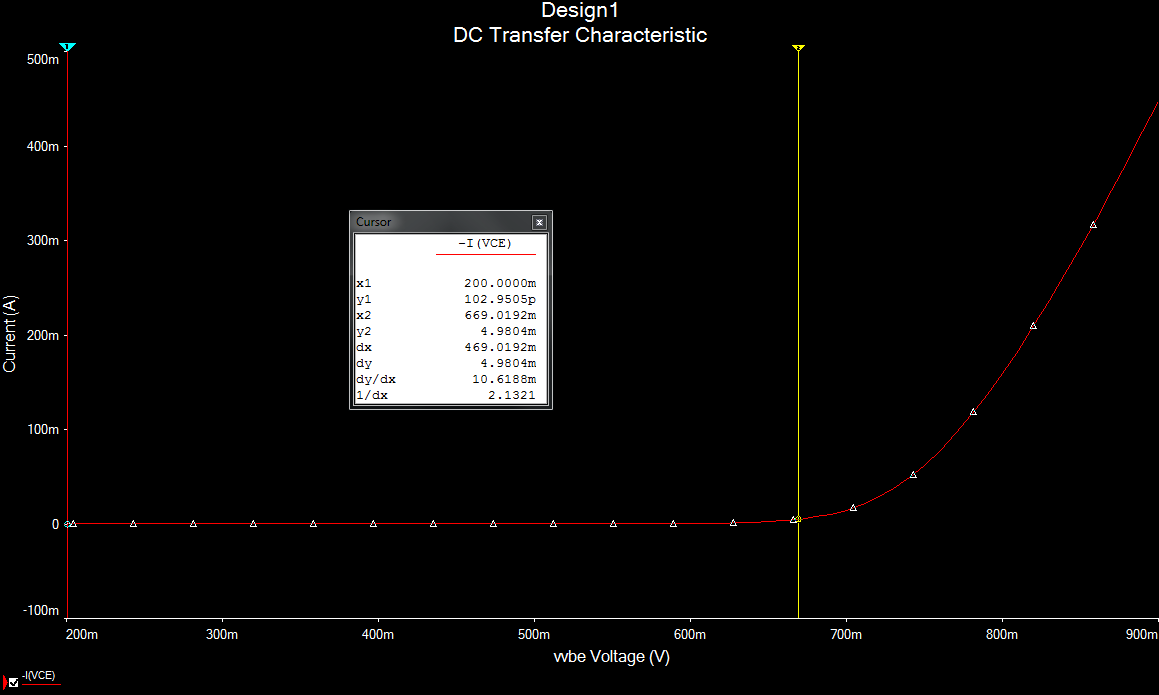
\includegraphics[height=1.75in]{pic3.PNG}


\section{Custom Models}
The custom model was a lot better than the one visualised here. The only problem was that due to memory leaks in the game and also running visual studio and 3ds max at the same time. The computer crashed while i was making the donald trump model twice, with me loosing all work. Thus the finalized model was a bit rushed.


\section{Fog}
Fog was implemented with the help of an online tutorial from http://in2gpu.com/2014/07/22/create-fog-shader/ this tutorial. The tutorial was quite useful and it was easy to apply these techniques to the already existing phong illumination vertex and fragment shaders. DUe to the phong illumination not being strong enough to properly display the fog effects with the background. A separate light source was added on top of the phong illumination to help it out 

\section{The video}

\begin{lstlisting}
https://www.youtube.com/watch?v=EGlBWtVR-2c&feature=youtu.be
\end{lstlisting}

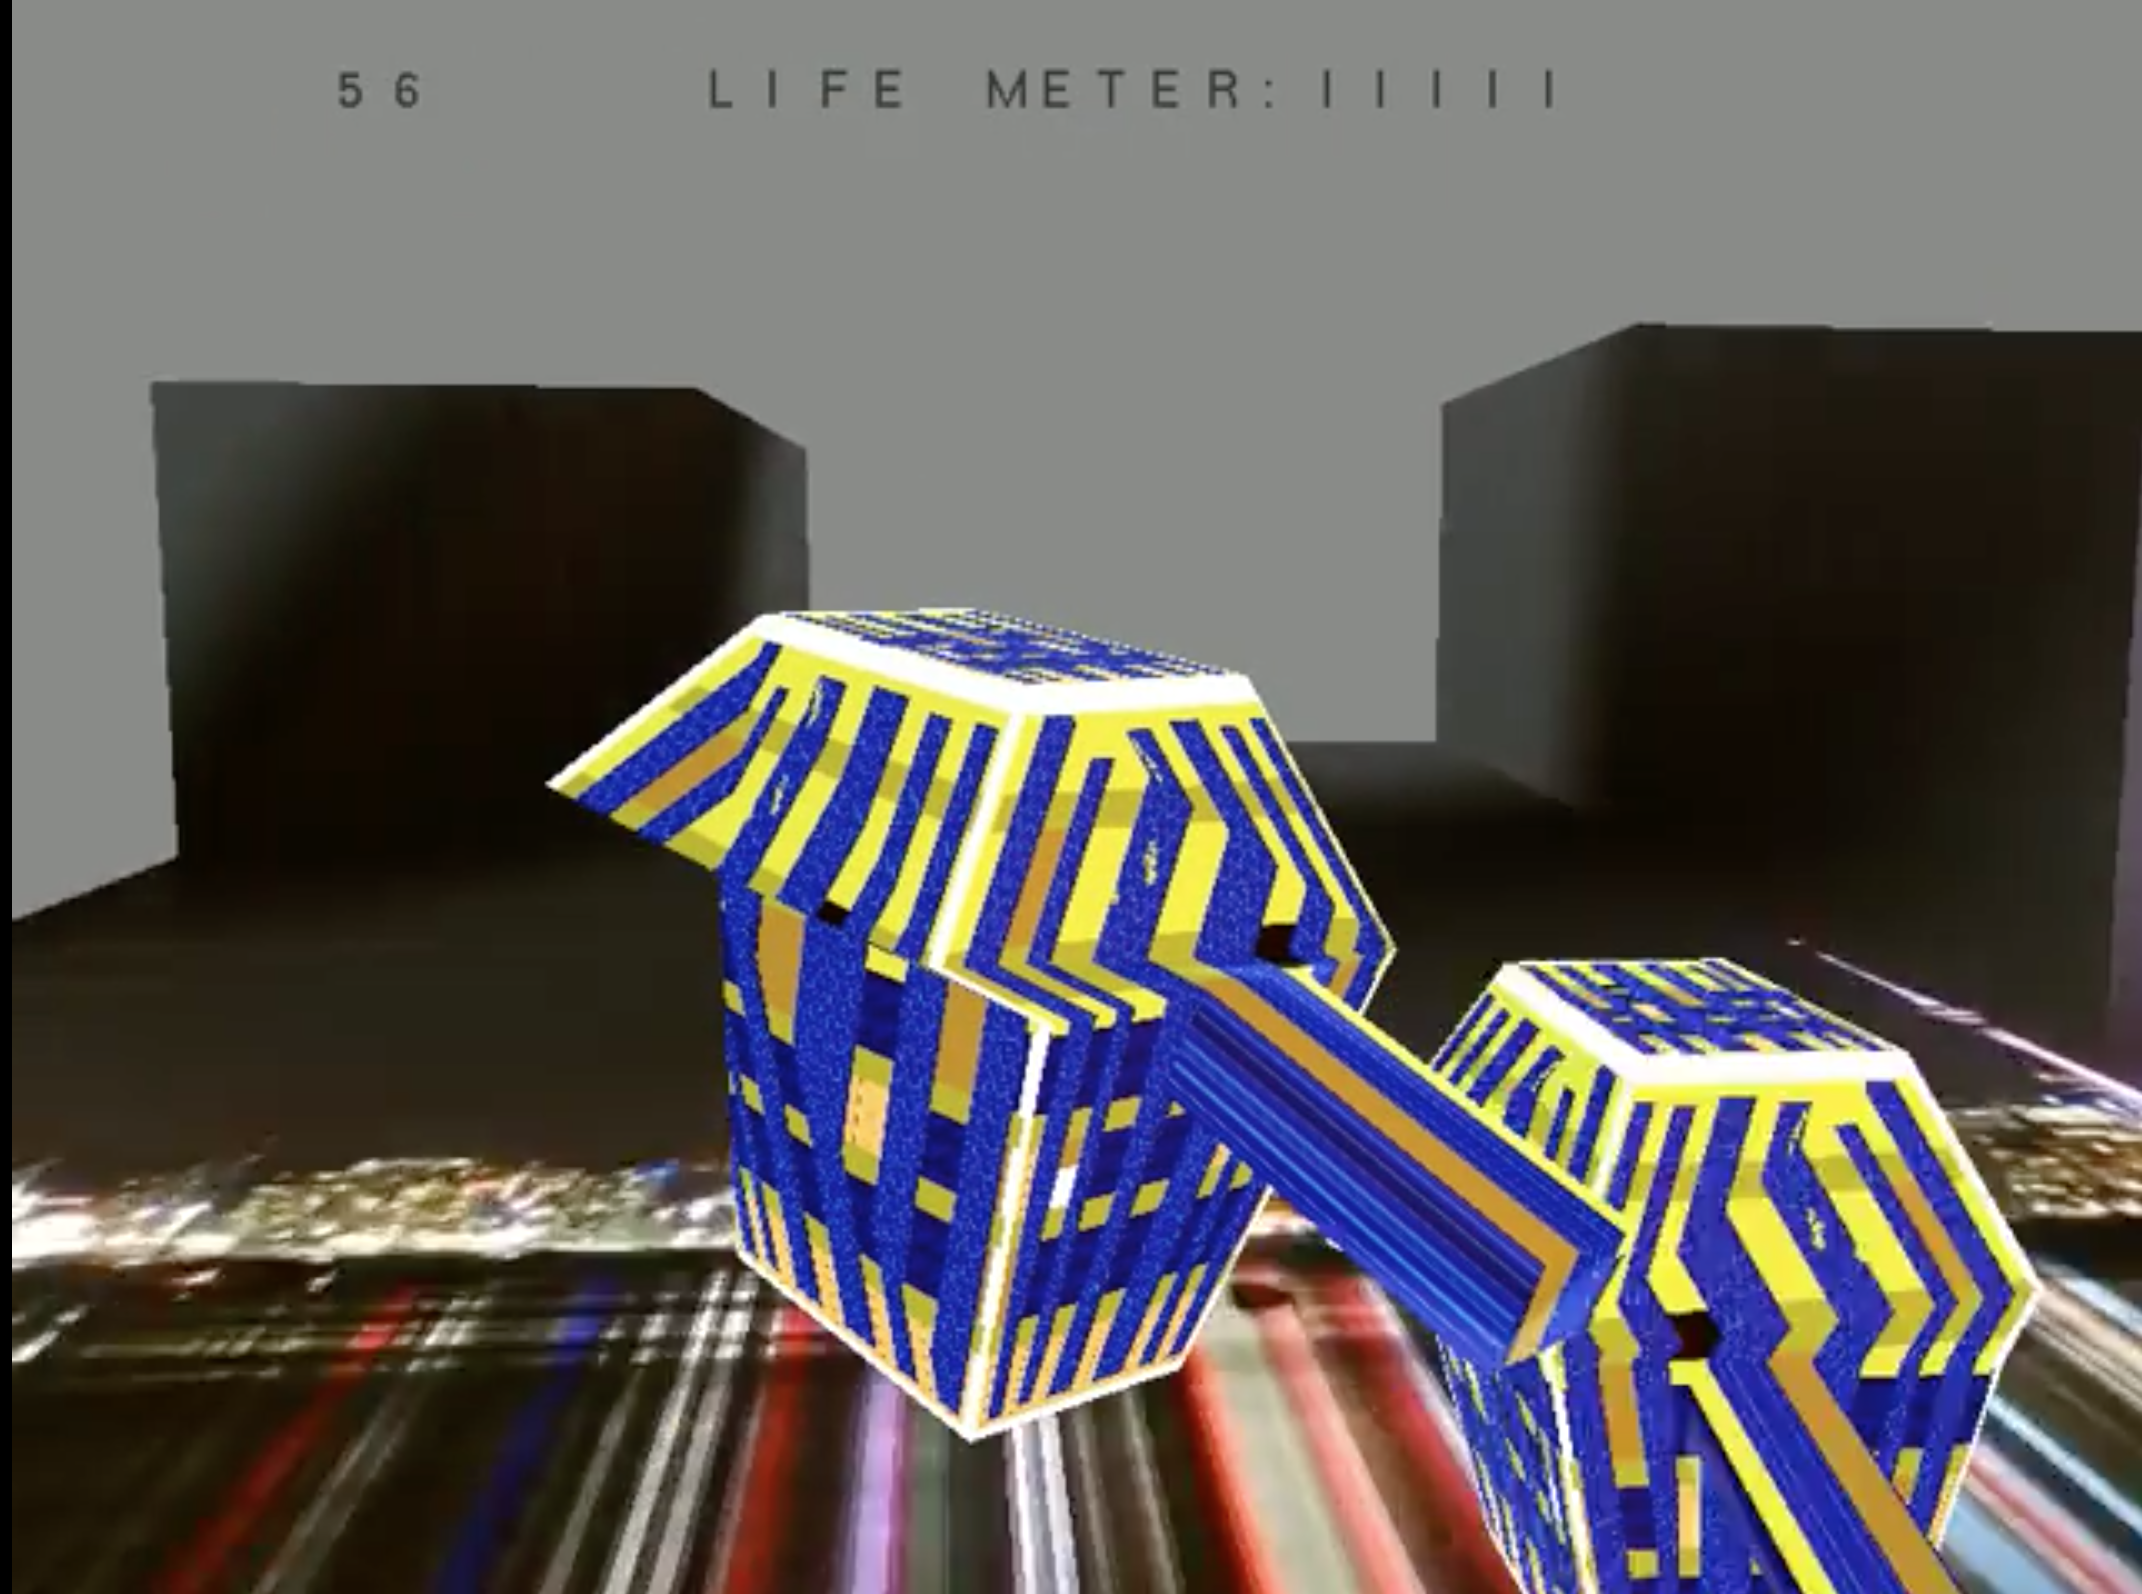
\includegraphics[height=1.75in]{pic1.PNG}


\pagebreak

	
\end{document}